\titleformat{\chapter}[display]{\bfseries\centering}{\huge Chapter \thechapter}{1em}{\Huge #1}
\newgeometry{top=3cm, bottom=2.2cm, left=3cm, right=2cm, headsep=1.2cm, footskip=1cm, headheight=0.3cm, textheight=24.5cm, textwidth=16cm}
\onehalfspacing
\pagestyle{fancy}
\fancyhf{}
\renewcommand{\headrulewidth}{0pt}
\lhead{Chapter 5}
\rhead{Results and Discussions}
\cfoot{\thepage}
\chapter{Results and Discussions}

\section{Application Results}
\noindent 16 of the 17 test cases in Table~\ref{tab:tests} passed. The one failure (TC-09) is a known weakness of the text model, explained in Section~\ref{sec:textres}. Figure~\ref{fig:res-harm} shows the harm results for a direct threat and for a quoted insult.

\begin{figure}[H]
\centering
\begin{minipage}[t]{0.62\linewidth}\centering
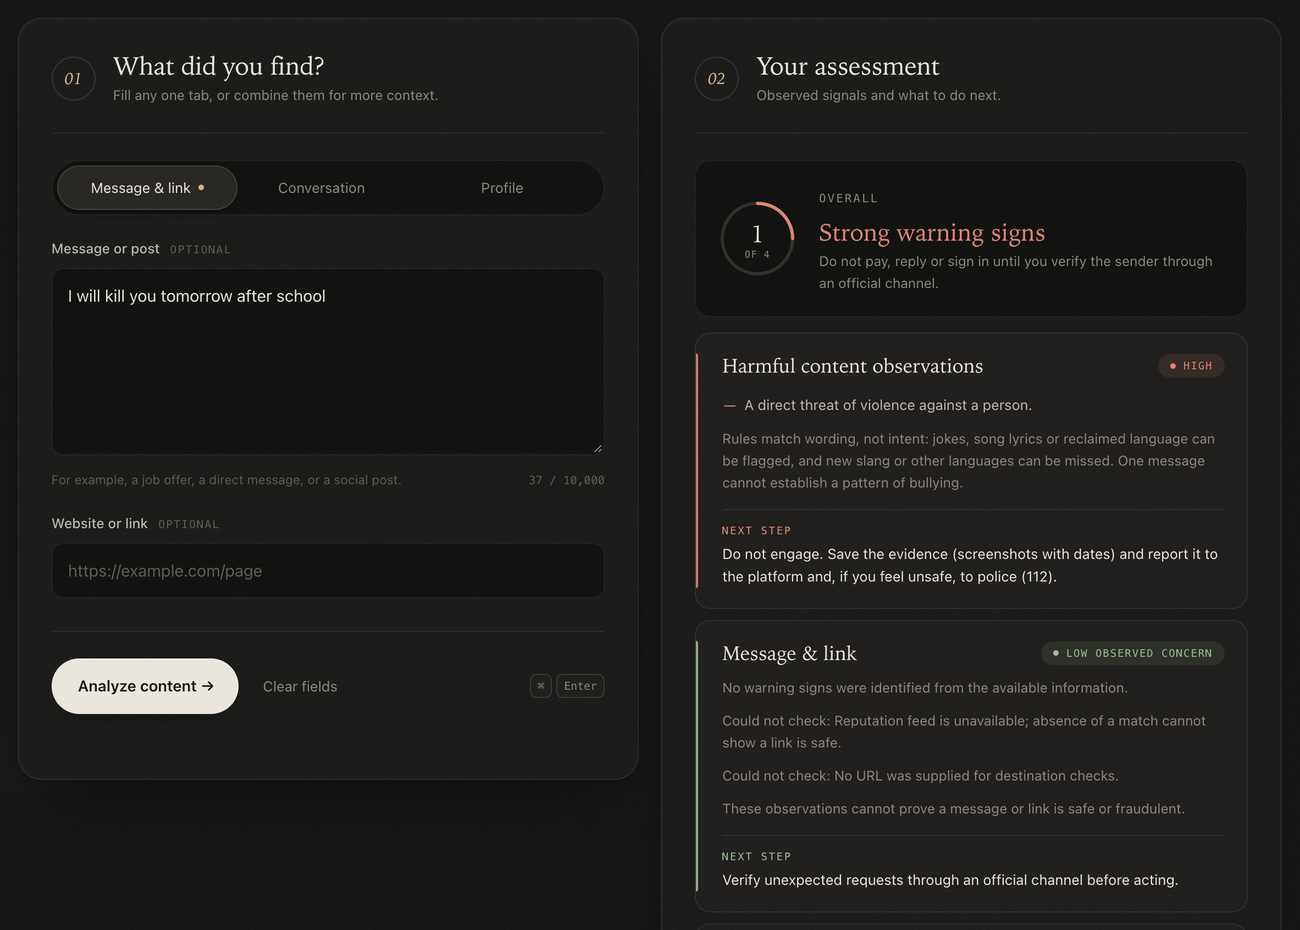
\includegraphics[width=\linewidth]{shots2/check_threat.png}\\[1pt]{\small (a) Direct threat: the harm card moves to the top}
\end{minipage}\hfill
\begin{minipage}[t]{0.30\linewidth}\centering
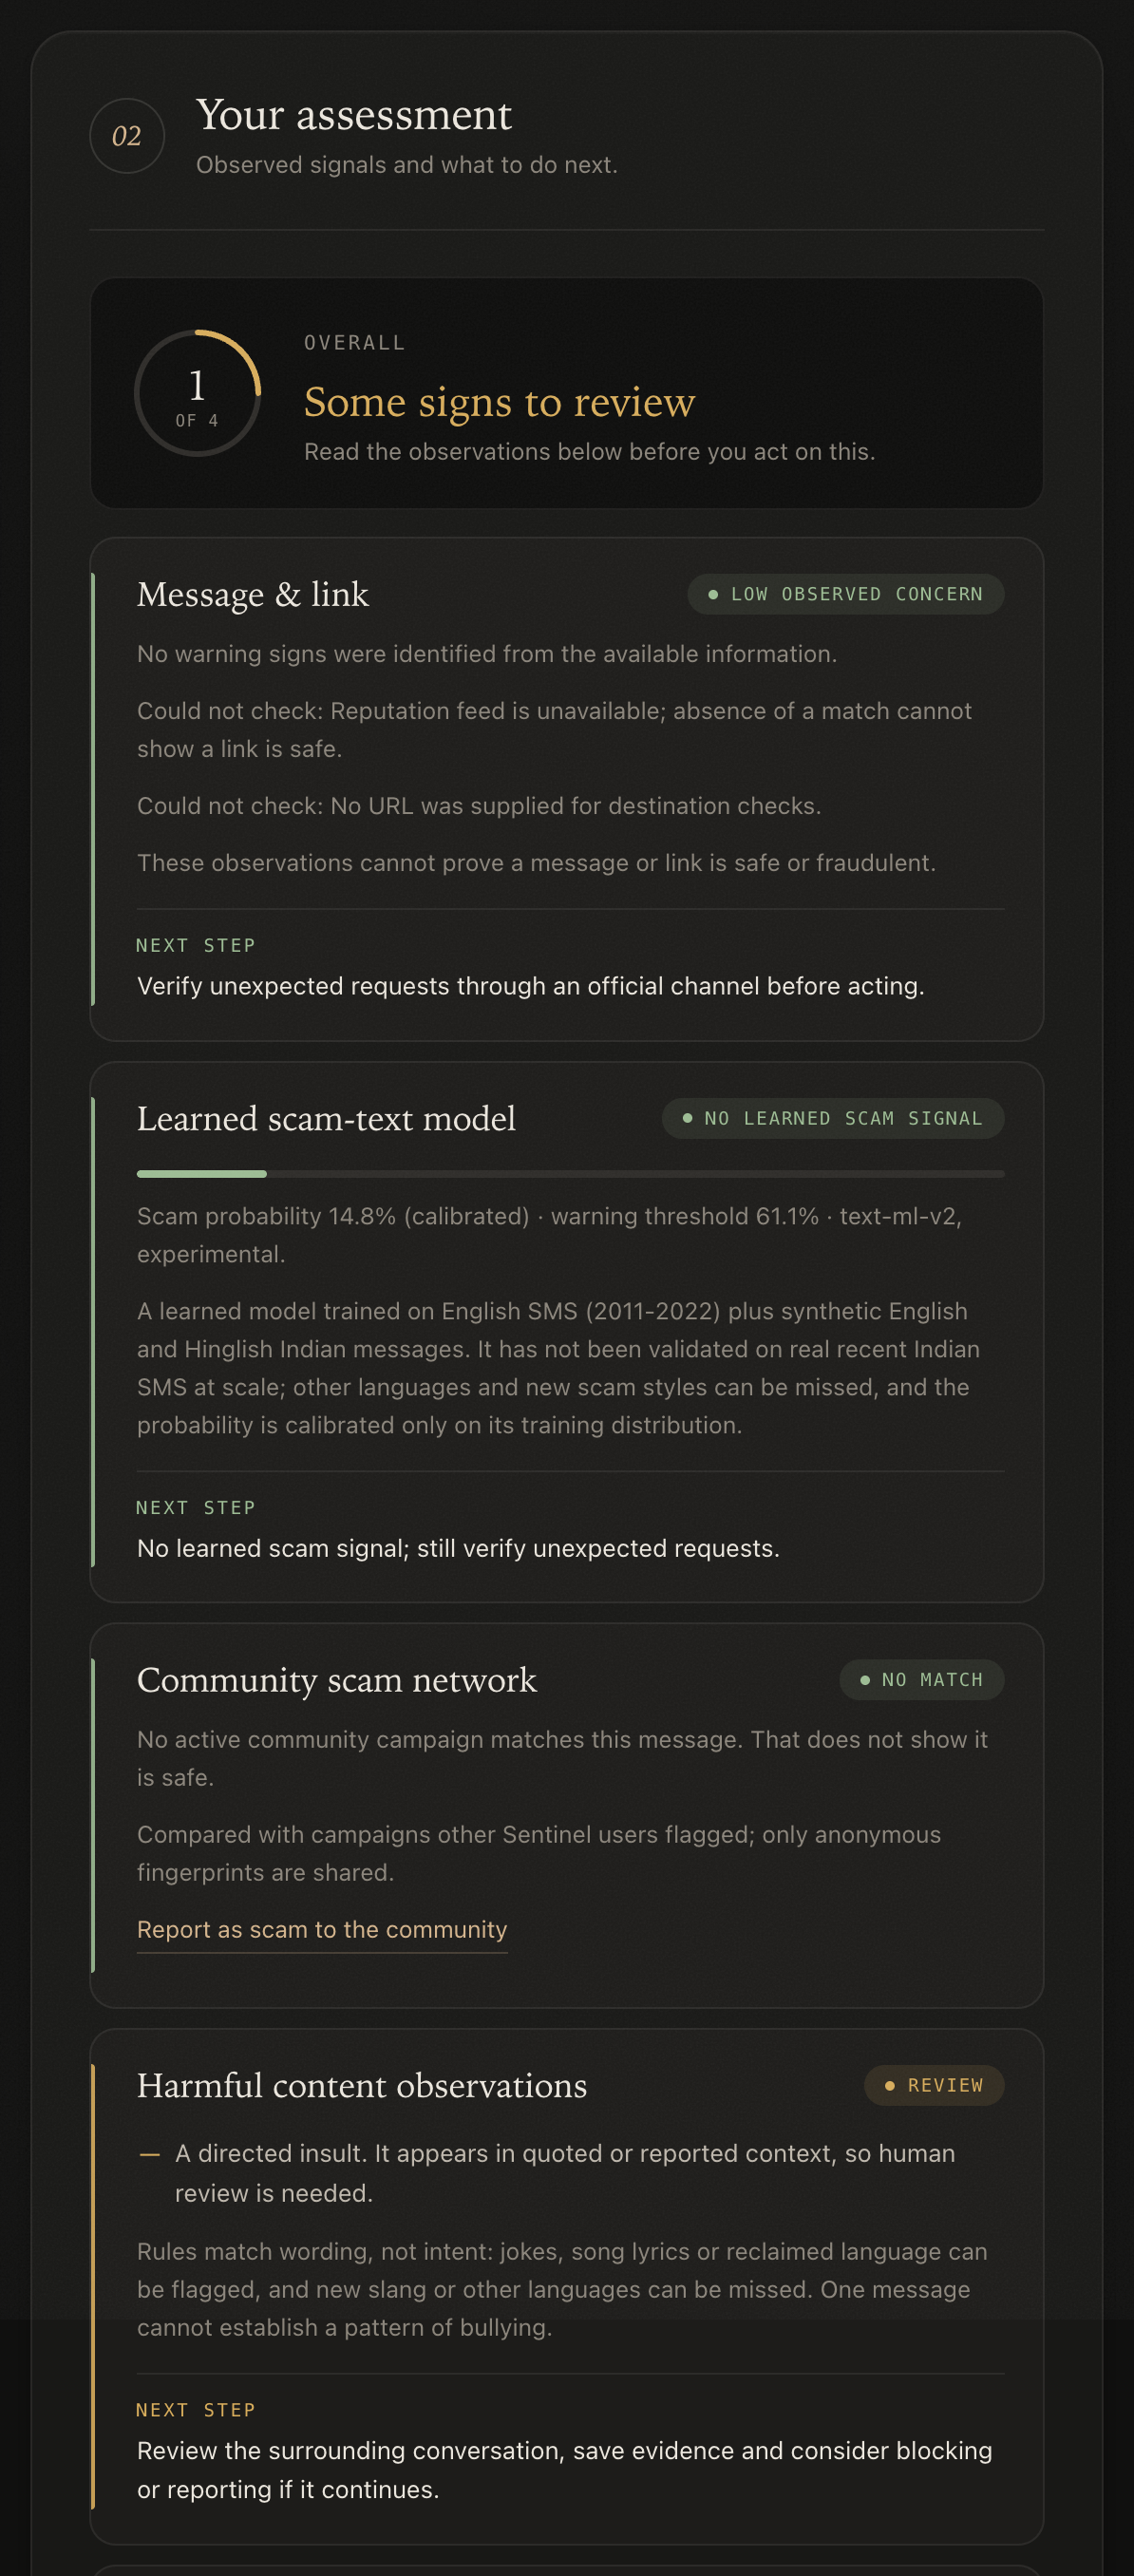
\includegraphics[width=\linewidth]{shots2/check_quoted.png}\\[1pt]{\small (b) Quoted insult: sent for human review}
\end{minipage}
\caption{Harmful-language results for a direct threat and a quoted insult}
\label{fig:res-harm}
\end{figure}

\noindent\textbf{Observations.}
\begin{itemize}
\item The fake internship (TC-01) was rated High by the rules, but the text model gave it only 56\%, below its 61.1\% threshold. This is why the model is shown \emph{next to} the rules and never replaces them.
\item Threats are rated High with clear advice; quoted insults go to human review instead of blaming the writer.
\item Rule checks finish in about a millisecond, so results feel instant.
\end{itemize}

\section{Scam-Text Model}\label{sec:textres}
\noindent Version 1 of the model scored well on its own test set, but our community-network simulation showed that it wrongly flagged 91--99\% of genuine Indian bank and OTP messages, because its training data had almost no genuine business messages. Version 2 added 2,000 Indian-style messages (synthetic) and averages two models. Table~\ref{tab:text} compares them.

\begin{table}[H]
\centering
\small
\renewcommand{\arraystretch}{1.15}
\caption{Scam-text model results}
\label{tab:text}
\begin{tabular}{|l|c|c|c|c|}
\hline
\textbf{Model} & \textbf{Macro-F1} & \textbf{Genuine flagged} & \multicolumn{2}{c|}{\textbf{Challenge set (44 msgs)}} \\
 & \textbf{(870 SMS)} & \textbf{(870 SMS)} & \textbf{Genuine flagged} & \textbf{Scams caught} \\ \hline
text-ml-v1 & 0.896 & 0 / 725 & 17 / 24 & 14 / 20 \\ \hline
\textbf{text-ml-v2} & \textbf{0.897} & \textbf{0 / 725} & \textbf{2 / 24} & \textbf{14 / 20} \\ \hline
\end{tabular}
\end{table}

\noindent Version 2 kept the same accuracy on the original test and cut false alarms on genuine Indian messages from 17 of 24 to 2 of 24. It runs in about 2 ms per message. \textbf{Limits:} the challenge set is small; the new data is synthetic; and the model still misses chat-style scams (``new number, send money'') and flags some genuine bank alerts.

\section{Harmful-Language Rules}
\noindent The old rule caught only 2 of 11 harmful test sentences. The new engine is tested on 12 high-risk sentences, 8 insults and 13 harmless sentences (idioms, negations and everyday Hinglish), and all are handled correctly. Because rules match words, not intent, new slang can still be missed.

\section{Auto-Scan Extension}
\noindent In TC-10 every page item got the expected severity. On the demo chat page the extension marked the job-fee, OTP and bank-login scams and the anonymous insult, and new messages were scanned as they appeared. A page scan takes about 190 ms. With image reading on, it also flagged the three scam images on the demo page, ignored the harmless one and read the link inside a QR code.

\section{Community Scam Network}
\noindent We simulated 10,000 users for 72 hours with 30 scam campaigns that are reworded every 6 hours and 12 genuine bulk messages.

\begin{table}[H]
\centering
\small
\renewcommand{\arraystretch}{1.15}
\caption{Share of scam messages that were warned}
\label{tab:net1}
\begin{tabular}{|l|c|c|}
\hline
\textbf{Detector on each device} & \textbf{Model alone} & \textbf{Model + network} \\ \hline
Simulated detector & 78.2\% & 99.7\% \\ \hline
text-ml-v2 (real model) & 86.0\% & 93.1\% \\ \hline
\end{tabular}
\end{table}

\begin{figure}[H]
\centering
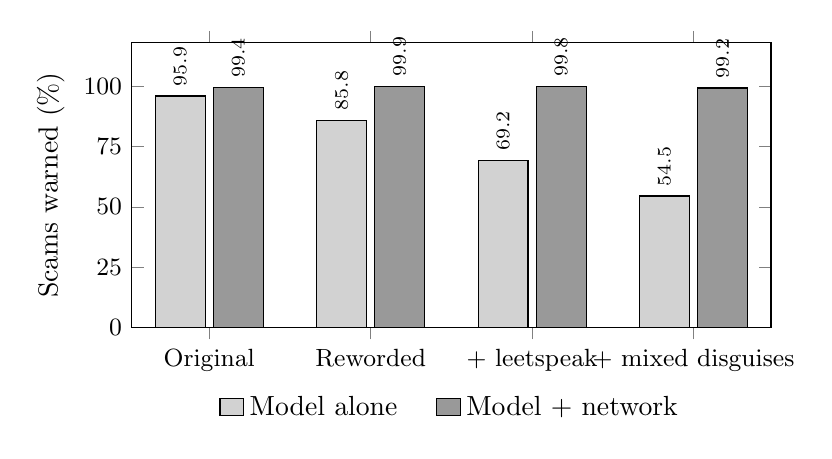
\begin{tikzpicture}
\begin{axis}[ybar=3pt, bar width=18pt, width=0.8\linewidth, height=5.2cm, ymin=0, ymax=118, ytick={0,25,50,75,100}, ylabel={Scams warned (\%)},
  symbolic x coords={Original,Reworded,+ leetspeak,+ mixed disguises}, xtick=data, enlarge x limits=0.16,
  legend style={at={(0.5,-0.2)}, anchor=north, legend columns=2, draw=none, /tikz/every even column/.append style={column sep=12pt}}, legend image code/.code={\draw[#1] (0cm,-0.1cm) rectangle (0.3cm,0.12cm);},
  nodes near coords, nodes near coords style={font=\scriptsize, rotate=90, anchor=west}, point meta=y,
  every axis plot/.append style={draw=black}, tick label style={font=\small}]
\addplot[fill=gray!35] coordinates {(Original,95.9) (Reworded,85.8) (+ leetspeak,69.2) (+ mixed disguises,54.5)};
\addplot[fill=gray!80] coordinates {(Original,99.4) (Reworded,99.9) (+ leetspeak,99.8) (+ mixed disguises,99.2)};
\legend{Model alone, Model + network}
\end{axis}
\end{tikzpicture}
\caption{Protection as scams get more disguised (simulated detector)}
\label{fig:netmut}
\end{figure}

\noindent As scams get more disguised, each user's own detector gets worse, but the network keeps protection near 99\% (Figure~\ref{fig:netmut}). The biggest risk we found was not attackers but honest mistakes at scale: a genuine message sent to thousands of people can collect several false reports. Without defences, 54.4\% of genuine bulk messages got a wrong warning; with the verified-sender list and user disputes, only 2.4\%. No message text was ever found in the hub's database.

\section{Bot-Account Detection}
\noindent Both trained models had to reach an AUC of at least 0.80 on \emph{every} dataset they had never seen (Table~\ref{tab:bot}).

\begin{table}[H]
\centering
\small
\renewcommand{\arraystretch}{1.15}
\caption{Bot models: results on unseen data}
\label{tab:bot}
\begin{tabular}{|>{\raggedright\arraybackslash}p{3.8cm}|>{\raggedright\arraybackslash}p{3.4cm}|c|c|c|}
\hline
\textbf{Model} & \textbf{Data} & \textbf{AUC, mixed data} & \textbf{Worst unseen AUC} & \textbf{Decision} \\ \hline
Profile model (bot-ml-v1) & 111,168 accounts, profile details & 0.967 & 0.600 & Failed: hidden \\ \hline
Activity model (bot-ml-activity-v1) & 10,422 accounts, posting behaviour & 0.997 & 0.849 & Passed: live \\ \hline
\end{tabular}
\end{table}

\noindent The profile model looked excellent on mixed data (0.967) but dropped to 0.600 on a dataset it had not seen, so it is not used. The activity model passed: it even caught human-like spambots it had never seen (AUC 0.981), where our hand-made score was worse than guessing (0.157). Its limit is that it learned from Twitter accounts of 2009--2017.

\section{URL Studies (Research Only)}
\noindent The first URL model reached 97.07\% F1 on PhiUSIIL, but all genuine URLs in that dataset were home pages, so the model learned the format rather than the fraud. The third model reached 92.71\% F1 on the larger PhreshPhish data, but still wrongly flagged 22.39\% of genuine links on a second test set (Figure~\ref{fig:v3}). Both are kept out of the application.
\begin{figure}[H]
\centering
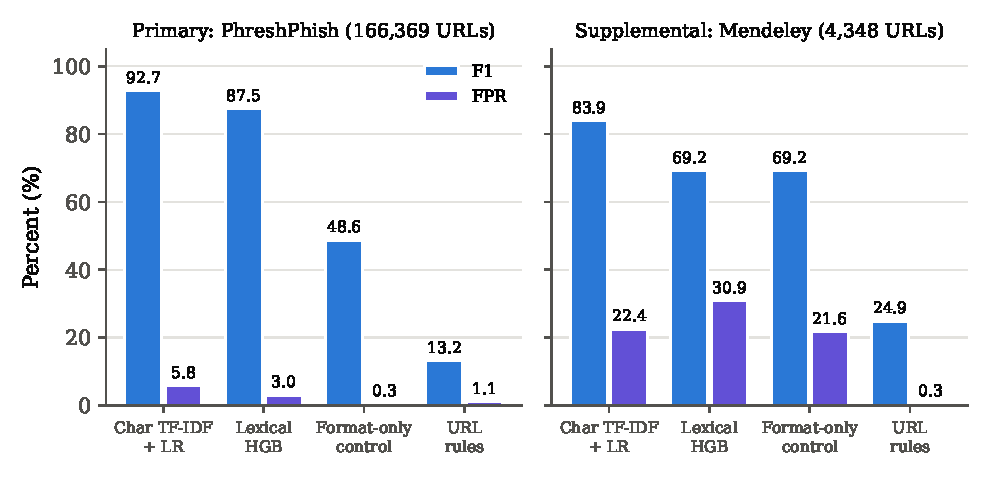
\includegraphics[width=0.78\linewidth]{charts/c5_v3_tracks.pdf}
\caption{URL model v3: F1 and false-positive rate on the two test sets}
\label{fig:v3}
\end{figure}
\noindent The message+link study has no real data yet, and the context-aware abuse study on CAD stopped because the data did not meet its minimum size rules, so no model was trained.

\section{Comparison with Existing Systems}
\begin{table}[H]
\centering
\small
\renewcommand{\arraystretch}{1.15}
\caption{Reported results of existing work and Sentinel (different tasks, shown for context)}
\label{tab:compare}
\begin{tabular}{|>{\raggedright\arraybackslash}p{3.6cm}|>{\raggedright\arraybackslash}p{4.2cm}|>{\raggedright\arraybackslash}p{5.6cm}|}
\hline
\textbf{System} & \textbf{Task} & \textbf{Result} \\ \hline
Aditya and Mohanty \cite{lit2} & Fake profiles (platform data) & 93.5\% accuracy \\ \hline
Atif et al. \cite{lit4} & Roman Urdu bullying & 97\% F1 \\ \hline
Sentinel text-ml-v2 & SMS scams & Macro-F1 0.897; 0 of 725 genuine flagged \\ \hline
Sentinel activity bot model & Twitter bots & Worst unseen AUC 0.849 \\ \hline
Sentinel URL v1 / v3 & Phishing URLs & 97.07\% / 92.71\% F1 (not live) \\ \hline
\end{tabular}
\end{table}
\noindent The tasks differ, so these numbers cannot be compared directly. Unlike the cited work, Sentinel tests on data its models have never seen. As Table~\ref{tab:features} shows, it is also the only system that combines all these checks, runs locally and explains its results.

\section{Discussion}
\noindent The application works as planned. Two learned models passed their tests and are live; two others failed and were kept out, which shows the testing process doing its job. The main lesson is that a high score is not enough: the URL model's 97\% and the profile bot model's 0.967 both hid weaknesses that only fair testing revealed.
